\tikzsetnextfilename{cooling}
\begin{frame}{From liquid to glass}
	\begin{columns}
	\column{0.6\textwidth}
	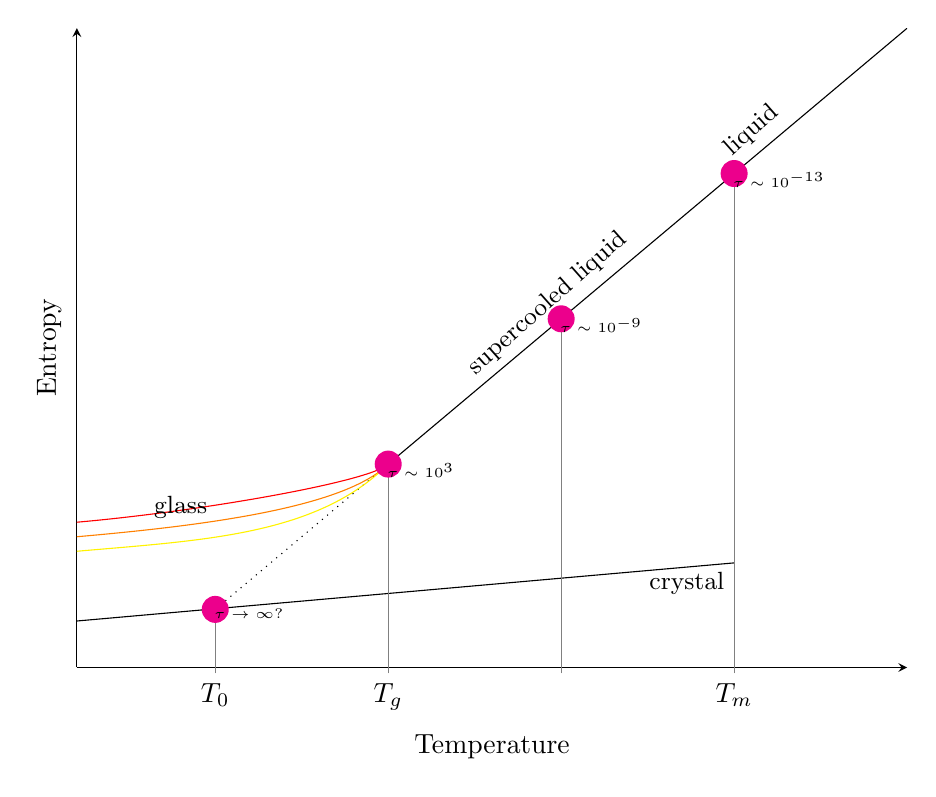
\begin{tikzpicture}[
		temp/.style={circle, inner sep=0.01\columnwidth, outer sep=0, fill=magenta},%
		label position=below right, label distance=-0.03\columnwidth,%
		]
	\begin{axis}[%
		width=\columnwidth, height=0.8\columnwidth,%
		xlabel=Temperature, xmin=0, xmax=1.2, axis x line=bottom, xtick=\empty,%
		extra x ticks={0.2, 0.45, 0.7, 0.95}, extra x tick labels={$T_0$, $T_g$,,$T_m$},%
		ylabel=Entropy, ymin=0.1, ymax=1.2, axis y line=left, ytick=\empty, ylabel near ticks,%
		]
		\draw (axis cs:0, 0.18) -- (axis cs:0.95, 0.28);
		\draw (axis cs:0.45, 0.45) -- (axis cs:1.2,1.2);
		\draw[dotted] (axis cs:0.2, 0.2)-- (axis cs:0.45, 0.45);
		\draw[help lines] (axis cs:0.2, 0)-- (axis cs:0.2, 0.2);
		\draw[help lines] (axis cs:0.45, 0)-- (axis cs:0.45, 0.45);
		\draw[help lines] (axis cs:0.7, 0)-- (axis cs:0.7, 0.7);
		\draw[help lines] (axis cs:0.95, 0)-- (axis cs:0.95, 0.95);
		\draw[red] (axis cs:0.45, 0.45) to [out=225, out looseness=0.2, in=5] (axis cs:0,0.35);
		\draw[orange] (axis cs:0.45, 0.45) to [out=225, out looseness=0.5, in=5] (axis cs:0,0.325);
		\draw[yellow] (axis cs:0.45, 0.45) to [out=225, out looseness=0.8, in=5] (axis cs:0,0.3);
		\node[temp, label=\tiny{$\tau\sim10^{-13}$}] at (axis cs:0.95, 0.95) {};
		\node[temp, label=\tiny{$\tau\sim10^{-9}$}] at (axis cs:0.7, 0.7) {};
		\node[temp, label=\tiny{$\tau\sim10^{3}$}] at (axis cs:0.45, 0.45) {};
		\node[temp, label=\tiny{$\tau\rightarrow\infty$?}] at (axis cs:0.2, 0.2) {};
		\node[above, anchor=south] at (axis cs:0.15, 0.34) (gl) {\small{glass}};
		\node[above, anchor=south, rotate=41.5] at (axis cs:0.7,0.7) {\small{supercooled liquid}};
		\node[above, anchor=south west, rotate=41.5] at (axis cs:0.95,0.95) {\small{liquid}};
		\node[below, anchor=north east] at (axis cs:0.95,0.28) {\small{crystal}};
	\end{axis}
	\end{tikzpicture}
	%\begin{footnotesize}\citet{cavagna2009supercooled}\end{footnotesize}
	\column{0.4\textwidth}
	\begin{itemize}
		\item Avoid crystallisation
		\item Slowing down by \alert{many} orders of magnitude
		\item A different type of solid: Glass
	\end{itemize}
	\end{columns}
	\begin{itemize}
		\item Kinetic glass transition $T_g$
		\item Not a thermodynamic transition but a dynamical arrest
	\end{itemize}
\end{frame}

\begin{frame}{Glass are amorphous}
	\begin{columns}
	\column{0.5\textwidth}
	Static structure factor
	\centering
	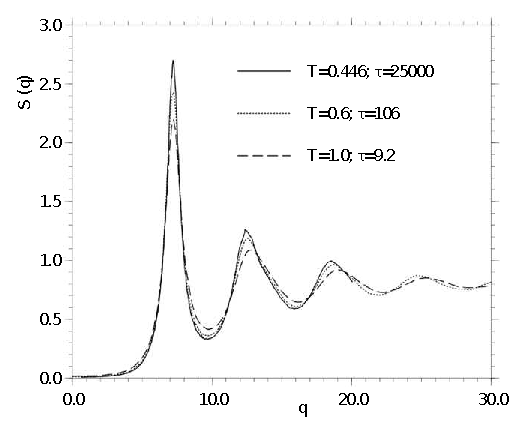
\includegraphics[width=\columnwidth]{sq_kob}
	
	{\footnotesize\citet{Kob2002}}
	
	\column{0.5\textwidth}
	While dynamics changes by 4 orders of magnitude
	\begin{itemize}
		\item Almost no change in positional order
		\item No characteristic length scale diverging toward $T_g$ or $T_0$
		\item $\neq$ critical phenomena
	\end{itemize}
	\end{columns}
\end{frame}

\tikzsetnextfilename{msd_kob}
\begin{frame}{Dynamics of supercooled liquids}

	{\footnotesize\citet{kob1995tmc}}
	\begin{columns}
	\column{0.4\textwidth}
	\centering
	\begin{tikzpicture}
		\node[above right] {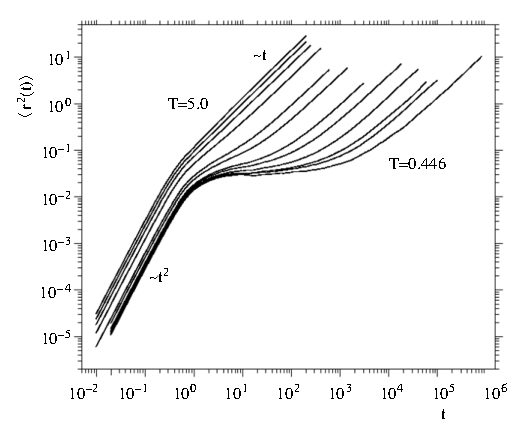
\includegraphics[width=0.95\columnwidth]{msd_kob}};
		\node at(0.9\columnwidth, 0.65\columnwidth) {$\alpha$};
		\node at(0.2\columnwidth, 0.35\columnwidth) {$\beta$};
	\end{tikzpicture}
	
	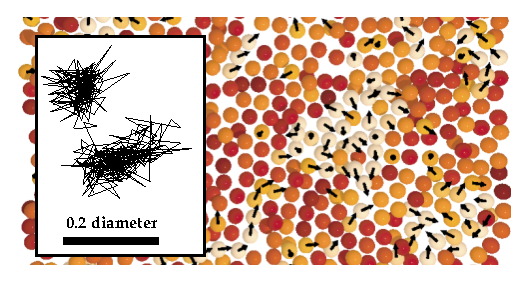
\includegraphics[width=\columnwidth]{cage_weeks}\\
	\column{0.55\textwidth}
	%Mean square displacement\\
	\begin{block}{Two step relaxation}
	\begin{itemize}
		\item A plateau appears
		\item $\beta$-relaxation does not change
		\item The length of the plateau changes\\ $\Rightarrow$ slowing down by many orders of magnitude
	\end{itemize}
	\end{block}
	\begin{block}{The cage theory}
	\begin{itemize}
		\item Hopping between cages $\ll\sigma$
		\item Is the hopping probability really uniform?
	\end{itemize}
	\end{block}
	\end{columns}
	{\footnotesize\citet{weeks2002pcr}}
\end{frame}

\begin{frame}{Dynamic is heterogeneous}
	\begin{columns}
	\column{0.4\textwidth}
	Fast and slow regions exist at intermediate times.
	\begin{center}
	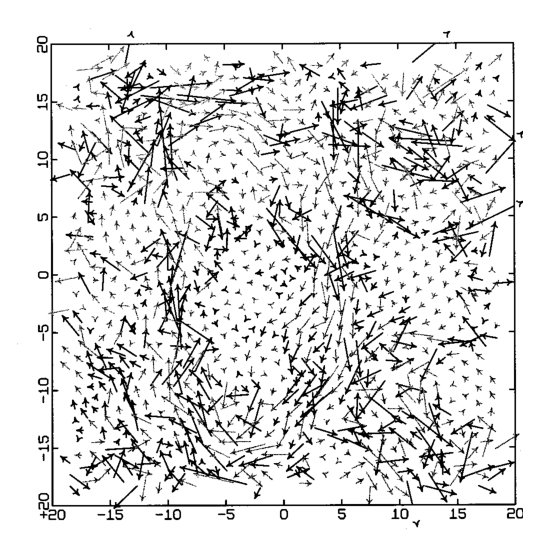
\includegraphics[width=\columnwidth]{dh_perera}\\
	{\footnotesize\citet{Perera1999}}
	\end{center}
	
	\column{0.6\textwidth}
	\begin{center}
	{\footnotesize\citet{Lacevic2003}}\\
	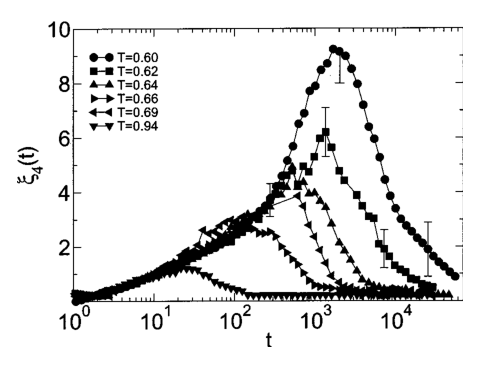
\includegraphics[width=0.7\columnwidth]{xi4_lacevic}
	\end{center}
	\begin{itemize}
		\item Spatial correlation of the fluctuations of the dynamics.
		\item Extract a dynamical correlation length
		\item Grows toward the glass transition
	\end{itemize}
	\end{columns}
\end{frame}
%\tikzset{external/force remake=true}
\begin{frame}{Dynamic vs static ?}\usebeamercolor{block title}
\alt<2>{\tikzsetnextfilename{dynamic_vs_static2}}{\tikzsetnextfilename{dynamic_vs_static1}}
\begin{flushright}
	\begin{tikzpicture}[concept/.style={scale=0.75, circle, font=\small, align=center, draw=bg, fill=bg, text width=6em, inner sep=0em}]
		\node[concept] (root2) {criticality};
		\node[below left=of root2, concept] (d2) {growing \alert{static} length scale};
		\node[below right=of root2, concept] (s2) {slowing down of global dynamics};
		\path (root2) to[circle connection bar switch color=from (bg) to (bg)] (d2);
		\path (root2) to[circle connection bar switch color=from (bg) to (bg)] (s2);
		\draw [thick, fg, ->] (d2) to [bend right] (s2);		
		
		\node[below right=0.15\textwidth and 0.3\textwidth of root2, concept] (root) {glass transition};
		\node[below right=of root, concept] (s) {slowing down of dynamics};
		\node[below=of root, concept] (d) {growing \alert{dynamic} length scale};
		\node<2>[below left=of root, concept] (sta) {growing \alert{static} length scale};
		\path (root) to[circle connection bar switch color=from (bg) to (bg)] (d);
		\path (root) to[circle connection bar switch color=from (bg) to (bg)] (s);
		\path<2> (root) to[circle connection bar switch color=from (bg) to (bg)] (sta);
		\draw[thick, dashed, fg, ->] (d) to [bend right] (s);
		\draw<2>[thick, dashed, fg, ->] (sta) to [bend right] (d);
	\end{tikzpicture}
\end{flushright}
\end{frame}%\tikzset{external/force remake=false}

\begin{frame}{Static cause to dynamic heterogeneities}
	\begin{columns}
	\column{0.5\textwidth}
	\centering
	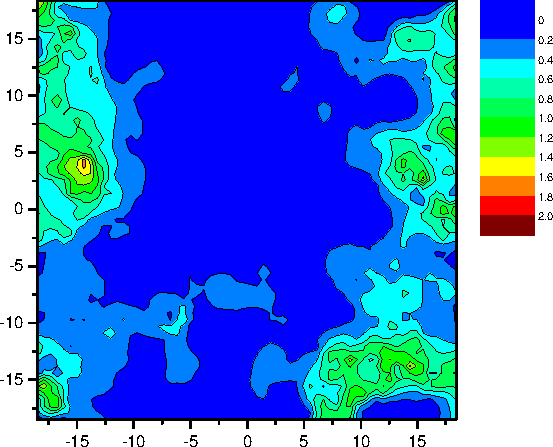
\includegraphics[width=\columnwidth]{propensity}
	\column{0.5\textwidth}
	{\footnotesize\citet{Widmer-Cooper2005}}
	\begin{itemize}
		\item $N$ runs from the same initial configuration
		\item Average out the influence of initial dynamics
		\item Propensity to displacement
		\item Predict fast/slow \alert{regions} ($>$~individual particle)\\{\footnotesize\citet{Berthier2007}}
	\end{itemize}
	\end{columns}
	
	\bigskip$\Rightarrow$ Glass transition may have a structural cause
\end{frame}

\tikzsetnextfilename{pentagons}
\begin{frame}{Candidates of structural order}
\small{Without long-ranged positional order}
\begin{columns}
\column{0.5\textwidth}
\begin{block}{Locally favoured structure (LFS) of the liquid}
Cannot fill space because of geometrical frustrations

\centering\begin{tikzpicture}[pen/.style={regular polygon, regular polygon sides=5, draw, minimum size=1cm}]
	\node[pen] (base) {};
	\node[pen,anchor=south, rotate=180] at (base.side 3) {};
	\node[pen,anchor=south, rotate=-108] at (base.side 4) {};
\end{tikzpicture}
\end{block}
Example: Icosahedron
\column{0.5\textwidth}
\centering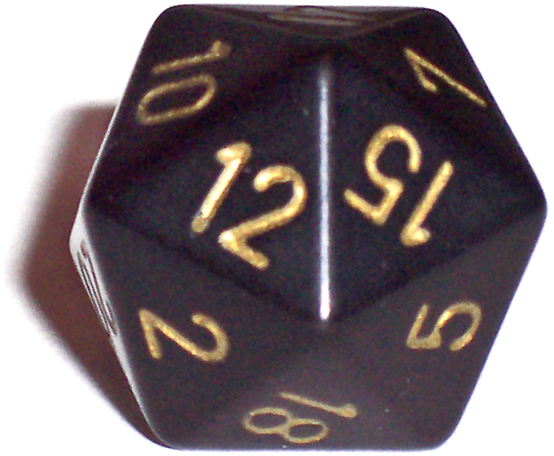
\includegraphics[width=0.5\textwidth]{d20.png}

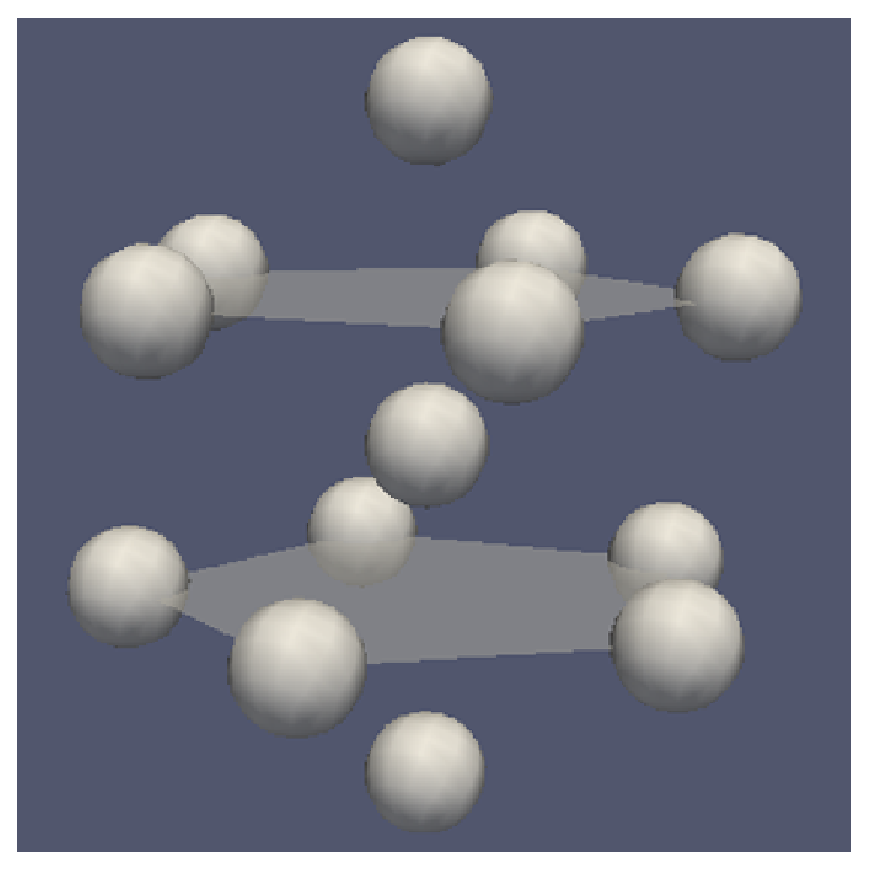
\includegraphics[width=0.5\textwidth]{ico_13}
\end{columns}
\end{frame}

\tikzsetnextfilename{hexagons}
\begin{frame}{Candidates of structural order}
\small{Without long-ranged positional order}
\begin{columns}
\column{0.5\textwidth}
\begin{block}{Influence of the crystal}
Cannot fill space because
\begin{itemize}
	\item Energy barrier
	\item Other structures locally more stable
	\item Kinetic barrier
	\item Size polydispersity
\end{itemize}
\end{block}
Example: Depends on the underlying crystal structure
\column{0.5\textwidth}
	\centering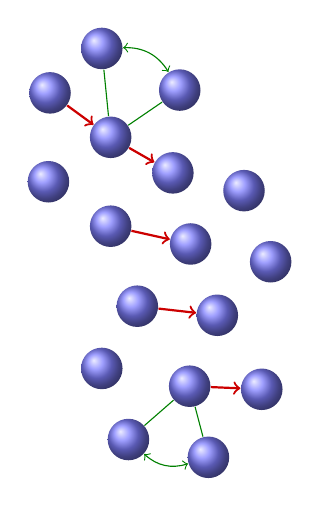
\begin{tikzpicture}[scale=0.2, rotate=-90]
		\tikzset{particle/.style={circle, ball color=blue!50!white, inner sep=0, minimum size=1.5em}}
		\tikzset{ar/.style={->, draw=red!80!black, thick}}
		\node[particle] at (14.356, 47.436) (a) {};
		\node[particle] at (17.000, 52.387) (b) {};
		\node[particle] at (20.000, 48.000) (c) {};
		\node[particle] at (17.178, 44.149) (d) {};
		\node[particle] at (22.258, 51.951) (e) {};
		\node[particle] at (22.822, 44.049) (f) {};
		\node[particle] at (23.387, 56.467) (g) {};
		\node[particle] at (27.902, 58.160) (g1) {};
		\node[particle] at (26.773, 53.080) (h) {};
		\node[particle] at (25.644, 48.000) (i) {};
		\node[particle] at (31.300, 54.773) (j) {};
		\node[particle] at (30.724, 49.693) (k) {};
		\node[particle] at (36.000, 57.596) (k1) {};
		\node[particle] at (35.804, 53.016) (l) {};
		\node[particle] at (34.676, 47.436) (m) {};
		\node[particle] at (40.320, 54.209) (n) {};
		\node[particle] at (39.191, 49.129) (o) {};
		\path[ar] (d) edge (c);
		\path[ar] (c) edge (e);
		\path[ar] (i) edge (h);
		\path[ar] (k) edge (j);
		\path[ar] (l) edge (k1);
		\draw[green!50!black] (a) -- (c) -- (b);
		\path[green!50!black,<->] (a) edge [bend left] (b);
		\draw[green!50!black] (n) -- (l) -- (o);
		\path[green!50!black,<->] (n) edge [bend left] (o);
	\end{tikzpicture}
\end{columns}
\end{frame}

\begin{frame}{Different structural cause $\Rightarrow$ different theory}
\begin{columns}[T]
\column{0.5\textwidth}
\structure{Liquid's order}
\begin{itemize}
	\item Spin-glass type\\{\footnotesize\citet{steinhardt1983boo}}
	\item Frustration-limited domain\\{\footnotesize\citet{tarjus2005fba}}
\end{itemize}
Icosahedral domain size\\
Defect size

\column{0.5\textwidth}
\structure{Crystal's order}
\begin{itemize}
	\item Tow order parameters\\{\footnotesize\citet{TanakaGJPCM}}
\end{itemize}

\bigskip
Bond order coherence length
\end{columns}
\begin{columns}
\column{0.5\textwidth}
\rotatebox{90}{\footnotesize \citet{Dzugutov2002}}
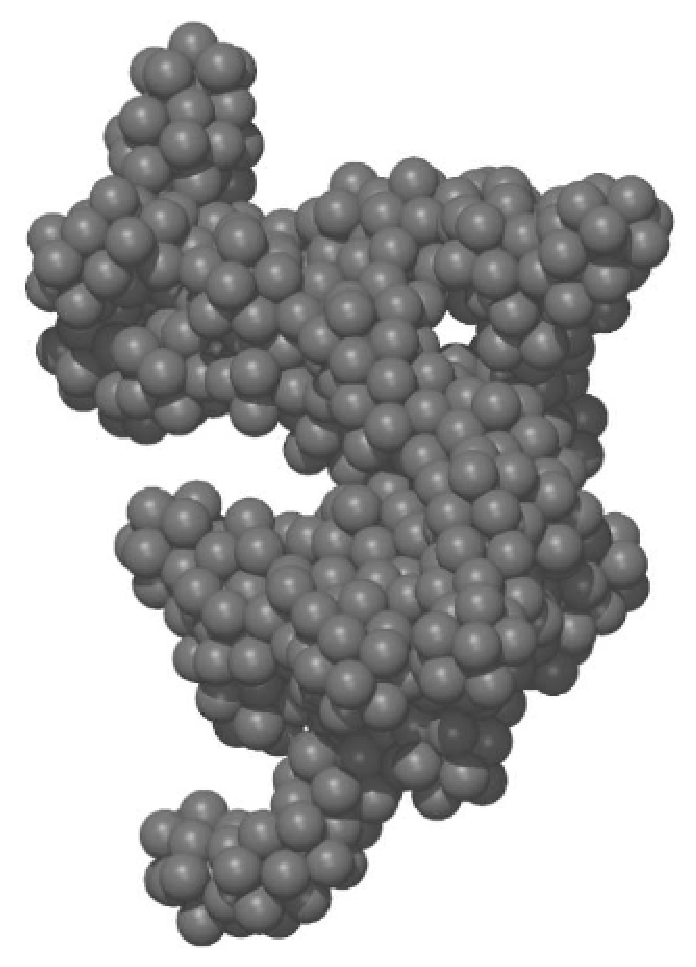
\includegraphics[width=0.5\columnwidth]{Dzugutov_LFS}
\column{0.5\textwidth}
\begin{tabular}{cc}
\resizebox{0.45\columnwidth}{!}{\input{kawa_nm_psi6.pdf_tex}} & \resizebox{0.45\columnwidth}{!}{\input{kawa_nm_msd.pdf_tex}} \\ 
$\Psi_6$ & $\Delta r^2$ \\ 
\end{tabular}
{\footnotesize\citet{tanaka2010critical}}
\end{columns}
\end{frame}

\begin{frame}{``Crystal'' is \ldots}
\ldots the symmetry breaking phase, avoided \alert{by definition} to get the supercooled liquid.
\begin{itemize}
	\item A classical crystal (\textsc{fcc, hcp, bcc}, \ldots)
\end{itemize}
\begin{columns}[T]
	\column{0.5\textwidth}
	\centering
	\begin{itemize}\item A quasi-crystal\end{itemize}
	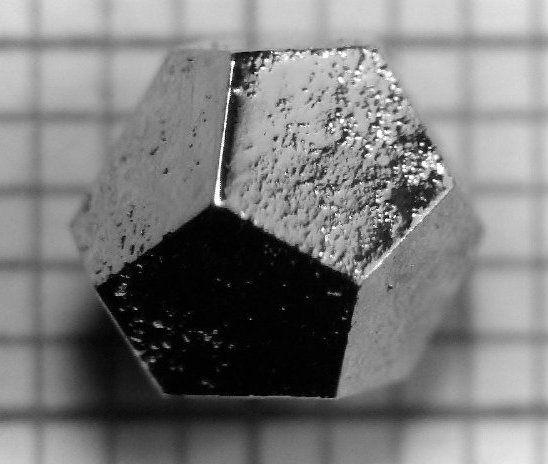
\includegraphics[height=0.5\columnwidth]{Ho-Mg-ZnQuasicrystal.jpg}\\
	{\footnotesize\citet{Doye2003}}
	\column{0.5\textwidth}
	\centering
	\begin{itemize}\item A Frank-Kasper phase\end{itemize}
	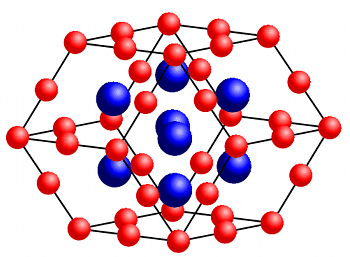
\includegraphics[height=0.5\columnwidth]{frankkasper.png}\\
	{\footnotesize\citet{Pedersen2010, Coslovich2011}}
\end{columns}

\bigskip
$\Rightarrow$ ``Crystal'' may contain icosahedral motif
\end{frame}

\begin{frame}{Slow icosahedral cluster means \dots}
\dots \alert{nothing} if the (quasi)crystalline state of the system has icosahedral motif.
\begin{itemize}
	\item Dodecagonal quasi-crystal for Dzugutov system\\{\footnotesize\citet{Doye2003}}
	\item Frank-Kasper phase for Wangstr\"om mixture\\{\footnotesize\citet{Pedersen2010, Coslovich2011}}
\end{itemize}

\begin{block}{We need a system}
\begin{itemize}
	\item With a known crystalline state $\nsupseteq$ icosahedral motif
	\item Exhibiting icosahedral order
\end{itemize}
\centering$\Longrightarrow$ Hard spheres
\end{block}
\end{frame}